\chapter{Creando un proyecto para Cypress FX2LP en Keil $\mu$Vision}
	\label{app:keil}
	El presente documento explica cómo configurar el Entorno de Desarrollo Integrado (IDE) Keil $\mu$Vision para poder desarrollar y compilar código para controladores FX2LP de Cypress.\\
	
	Se entiende por IDE a un software que integra en un entorno gráfico las herramientas que permiten elaborar un programa que ejecutará un procesador, desde la escritura del algoritmo en uno o más lenguajes, las pruebas, el depurado y el compilado del mismo.\\
	
	\begin{figure}[ht]
		\centering
		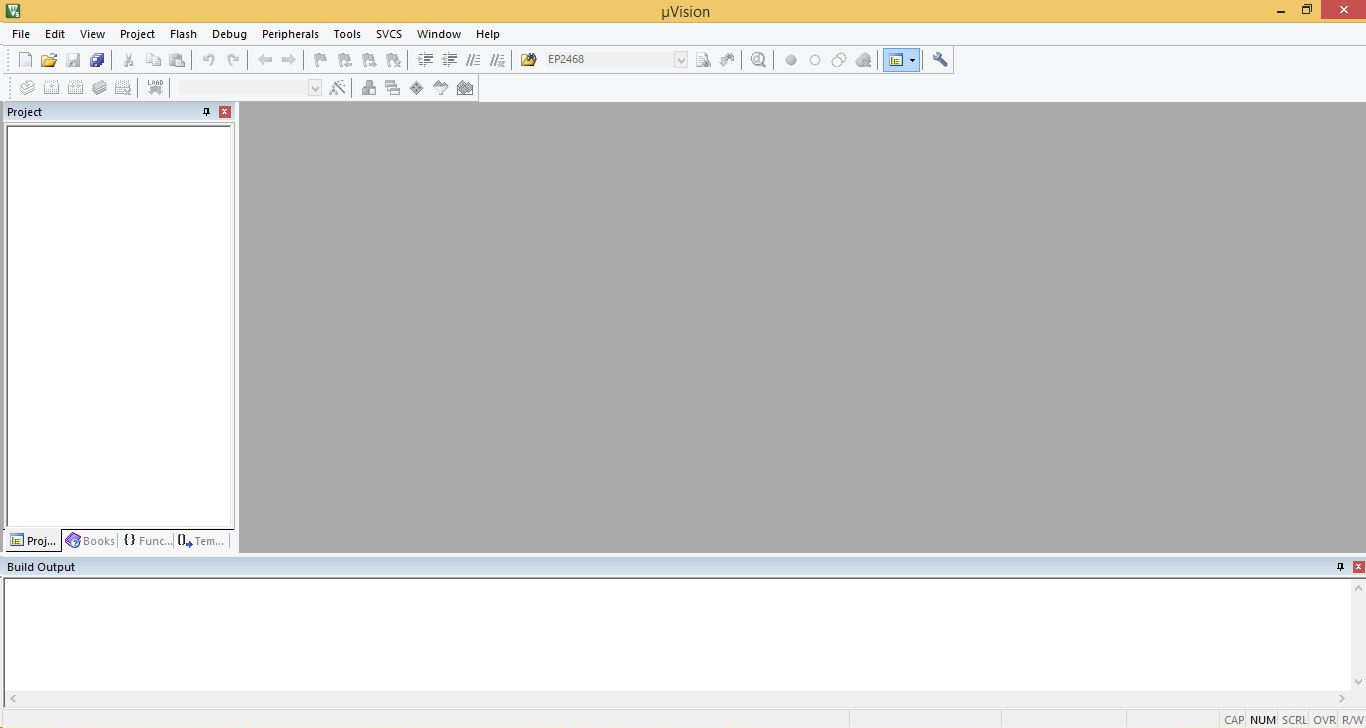
\includegraphics[width=0.7\textwidth]{A1keil.png}
		\caption{Vista inicial de la ventana de Keil $\mu$Vision}
		\label{initkeil}
	\end{figure}
	Cuando el usuario inicia el programa, se encuentra con una ventana como la que se observa en la Figura \ref{initkeil}.